%!TEX TX-program = xelatex
%
%%%%%%%%%%%%%%%%%%%%
%
% Title: GCSE Mathematics & Additional Mathematics for 23.08.22
% Author: Eason Shao, Mr Finch-Noyes
% Date: 23.08.22
% Institude: Oxford International College
% Email: eason.syc@icloud.com; yicheng_shao@oxcoll.com
% GitHub: https://github.com/EasonSYC
% GitHub Repository: https://github.com/EasonSYC/GCSE-Maths-Notes
%
%%%%%%%%%%%%%%%%%%%%

\documentclass[8pt]{article}
\usepackage{../allan-eason}

\usetikzlibrary{positioning}
\usetikzlibrary{svg.path}

\graphicspath{ {./images/} }

\newcommand{\Date}{23.08.22}
\newcommand{\Name}{Mathematics}
\newcommand{\Title}{\textcolor{allandarkblue}{\Name}\ \textcolor{allancyan}{\Date}\ Notes}

\newcommand{\Author}{Eason Shao, Mr Finch-Noyes}

\author{\Author}
\title{\Title}
\date{\Date}

\geometry{a4paper, scale=0.8}

\lhead{\Title}

\begin{document}

	\maketitle

	\tableofcontents

	\section{Converting Between Decimals and Fractions}

		\exmp Write \(-7\) as a fraction. \(-7 = -7 / 1\).

		\exmp Write \(2.9\) as a fraction. \(2.9 = 29/10\).

		\exmp Write \(-37.081\) as a fraction. \(-37.081 = -37081/1000\).

		\exmp Write \(0.\dot{3}\) as a fraction. \(0.\dot{3} = 3 / 9 = 1 / 3\).

		\exmp Write \(0.\dot{1}\) as a fraction. \(0.\dot{1} = 1 / 9\).\newline

		\prob Write \(0.\dot{7}\) as a fraction.
		
		\solution \(0.\dot{7} = 7 / 9\).\newline

		\meth \methword{(Converting decimals to fractions)} Let \(x = 0.\dot{3}\), thus \(10x = 3.\dot{3}\). Therefore \(10x - x = 3.\dot{3} - 0.\dot{3} = 3 = 9x\), and \(x = 3/9 = 1/3\).\newline

		\prob Show that \(2.1\dot{5}\dot{7} \in \QQ\).
		
		\solution Let \(x\) be \( 2.1 \dot{5} \dot{7}\), therefore \(10x = 21.\dot{5}\dot{7}, 1000x = 2157.\dot{5}\dot{7}\).
		
		\(1000x - 10x = 2136 = 990x, x = 2136/990 = 178/75 \in \QQ\).\newline

		\prob Express \(x = -62.\dot{0}3\dot{2}\) as a fraction.
		
		\solution \(1000x = -62032.\dot{0}3\dot{2}, 1000x - x = 999 x = -61970, x = 61970 / 999\). \newline

		\prob Express \(x = 82.\dot{8}5714\dot{2}\) as a fration.
		
		\solution \(x = 82\frac{6}{7} = 580/7\).

	\section{Sets}

		\exmp Let Universal Set be \(\mathscr{E} = \left\{1, 2, 3, 4, 5, 6, 7, 8, 9, 10\right\}\). Let \(E\) be the set of evens, \(R\) be the set of primes, \(D\) be the set of odds, \(T := \{2, 3\}\). Write in a Venn Diagram. \(E = \{2, 4, 6, 8, 10\}; R = \{2, 3, 5, 7\}; D = \{1, 3, 5, 7, 9\}\).

		\[
		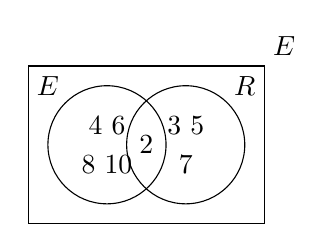
\begin{tikzpicture}
			\draw[black] (0, 0)--(3, 0)--(3, 2)--(0, 2)--(0, 0);
			\draw[black] (1, 1) circle [radius = 0.75];
			\draw[black] (2, 1) circle [radius = 0.75];
			\node at (1.5, 1) {\(2\)};
			\node at (1, 1.25) {\(4\ 6\)};
			\node at (1, 0.75) {\(8\ 10\)};
			\node at (2, 1.25) {\(3\ 5\)};
			\node at (2, 0.75) {\(7\)};
			\node at (0.25, 1.75) {\(E\)};
			\node at (2.75, 1.75) {\(R\)};
			\node at (3.25, 2.25) {\(\mathscr{E}\)};
		\end{tikzpicture}
		\]

		\exmp \exmpword{(Intersection)} \(E\cap R = \left\{2\right\}\).

		\exmp \exmpword{(Union)} \(E \cup R = \left\{2, 4, 6, 8, 10, 3, 5, 7\right\}\).

		\exmp \exmpword{(Complement)} \(R^{\prime} = \{4, 6, 8, 10, 1, 9\}\).

		\exmp \exmpword{(Empty Set)} \(D \cap E = \emptyset\).

		\exmp \exmpword{(In)} \(3 \in R\) is True. \(3\) is an element of \(R\).

		\exmp \exmpword{(Not In)} \(4 \notin R\) is True. \(4\) is not an element of \(R\).

		\exmp \exmpword{(Proper Subset)} \(T \subset R (T \notin R)\).

		\exmp \exmpword{(Subset)} \(R \subseteq R (R \not \subset R)\).

		\exmp \exmpword{(Number)} \(\mathrm{n}(R) = 4\). Number of elements in \(R\) is \(4\).\newline

		\prob Simplify \(R \cup E^{\prime}\).
		
		\solution
		
		\begin{align*}
			R \cup E^{\prime} &= \{2, 3, 5, 7\} \cup \{2, 4, 6, 8, 10\}^{\prime}\\
			&= \{2, 3, 5, 7\} \cup \{1, 3, 5, 7, 9\}\\
			&= \{1, 9, 3, 5, 7, 2\}.
		\end{align*}

		\prob Simplify \(T^{\prime} \cup E\).
		
		\solution
		
		\begin{align*}
			T^{\prime} \cup E &= \{2, 3\}^{\prime} \cup \{2, 4, 6, 8, 10\}\\
			&= \{1, 4, 5, 6, 7, 8, 9, 10\} \cup \{2, 4, 6, 8, 10\}\\
			&= \{1, 2, 4, 5, 6, 7, 8, 9, 10\}.
		\end{align*}

		\prob Simplify \(T^{\prime} \cap E\)
		
		\solution
		
		\begin{align*}
			T^{\prime} \cap E &= \{2, 3\}^{\prime} \cap \{2, 4, 6, 8, 10\}\\
			&= \{1, 4, 5, 6, 7, 8, 9, 10\} \cap \{2, 4, 6, 8, 10\}\\
			&= \{4, 6, 8, 10\}.
		\end{align*}

		\prob Simplify \(\mathrm{n} \left(T^{\prime} \cap R\right)\).
		
		\solution
		
		\begin{align*}
			\mathrm{n} \left(T^{\prime} \cap R\right) &= \mathrm{n} \left(\{2, 3\}^{\prime} \cap \{2, 3, 5, 7\}\right)\\
			&= \mathrm{n} \left(\{1, 4, 5, 6, 7, 8, 9, 10\} \cap \{2, 3, 5, 7\}\right)\\
			&= \mathrm{n} \{5, 7\}\\
			&= 2.
		\end{align*}

		\prob Simplify \(R^{\prime} \cup \left(E \cap T\right)\).
		
		\solution
		
		\begin{align*}
			R^{\prime} \cup \left(E \cap T\right) &= \{2, 3, 5, 7\} \cup \left(\{2, 4, 6, 8, 10\} \cap \{2, 3\}\right)\\
			&= \{1, 4, 6, 8, 9, 10\} \cup \{2\}\\
			&= \{1, 4, 6, 8, 9, 10, 2\}.
		\end{align*}

		\prob Simplify \(\left(E \cup T\right)^{\prime}\).
		
		\solution
		
		\begin{align*}
			\left(E \cup T\right)^{\prime} &= \left(\{2, 4, 6, 8, 10\} \cup \{2, 3\}\right)^{\prime}\\
			&= \{2, 3, 4, 6, 8, 10\}^{\prime}\\
			&= \{1, 5, 7, 9\}.
		\end{align*}

		\prob Simplify \(R^{\prime} \cup T\).
		
		\solution
		
		\begin{align*}
			R^{\prime} \cup T &= \{1, 4, 6, 8, 9, 10\} \cup \{2, 3\}\\
			&= \{1, 2, 3, 4, 6, 8, 9, 10\}.
		\end{align*}

\end{document}